\documentclass[10pt,a4paper]{book}
\usepackage[utf8]{inputenc}
\usepackage[T1]{fontenc}
\usepackage{amsmath}
\usepackage{amsfonts}
\usepackage{amssymb}
\usepackage{graphicx}
\usepackage[cache=false]{minted}
\usemintedstyle{colorful}
%\definecolor{bg}{HTML}{282828} % from https://github.com/kevinsawicki/monokai
%\setminted{bgcolor=bg,breaklines=true}
\setminted{breaklines=true}
\begin{document}
\title{Data Structures}
\author{Andrew Rosen}
\date{}
\maketitle
\tableofcontents

\part{Preliminaries}

\chapter{Introduction}

\section{What is a Data Structures Course}
Data Structures is all about defining the different ways we can organize data.


\section{Why This Book?}

This text


\subsection{Where Does This Book Fit Into a Computer Science Curriculum }

Education in Computer Science is based around three core topics: translating the steps of solving a problem into a language a computer can understand, organizing data for solving problems, and techniques that can be used to solve problems. % reword
These courses typically covered in a university's introductory course, data structures course, and algorithms course respectively, although different universities decide exactly what content fits in which course.
Of course, there is are lot more concepts in computer science, from operating systems and low level programming,  to networks and how computers talk to each other. However, all these concepts rely on the knowledge gained in the core courses of programming, data structures, and algorithms.

 

This textbook is all about Data Structures, the middle section between learning how to program and the more advanced problem solving concepts we learn in Computer Science. 
Here, we focus on mastering the different ways to organize data, recognize the internal and performative differences between each structure, and learn to recognize the best (if there is one) for a given situation.


\subsection{What Are My Base Assumptions about the Reader?}

This textbook assumes that the student has taken a programming course that has covered the basics.
Namely: data types such as ints, doubles, booleans, and strings; if statements, for and while loops; and object orient programming.
This book is also suitable for the self taught programmer who has not learned much theoretical programming

\section{To The Instructor}

You'll note that this textbook lacks many of the 



Does the lack of varied exercises make cheating on assignments easier as semesters go on?  Yes, but that bridge was burned long ago.  
The cheating student can plagarize from various websites or anonymously hire another to do their work for them.
However, the student who cheats isn't exactly clever and certainly hasn't been exposed to much game theory.  
They will often cheat from the same source.  




\section{To The Student}


%\section{Science and Art}


\chapter{Functions and How They Work}

This will be an extremely short chapter, but an important one.

\section{The Runtime Stack}


\section{Passing Arguments}

\subsection{How it Works in Java}

\subsection{How it works in Python}


\chapter{The Array}

\section{Why Arrays}

\begin{itemize}
	\item because new language: 
	Since this is a data structures course, I assumed that students have had exposure to arrays or array like objects.
	This chapter goes into a bit of a deeper detail that may have been glossed over and Introduces the topic in the appropriate language if need be.
	
	In other words, I assume you know what an array is , but not necessarily how to use it in Java or Python\footnote{Although we use lists in python}.
	\item  because internal memory lookup
	\item Becuase we need to make sure internal knowledge is cohesive (eg arrays of objects are arrays of pointers/references)
\end{itemize}







\section{Java and Arrays}
The Array is a built in class in Java, but the syntax is a bit unique \footnote{Enough so that I constantly had to look up how to do it my first two years of undergraduate studies, so don't feel too bad if you have to do the same}

To create an array in Java we do:

\begin{minted}{Java}
Type[] myArray = new Type[sizeOfArray]
\end{minted}


Here, every item in the array is of whatever \texttt{Type} we want, which could be a Class or primitive.   
Arrays can be whatever integer size we desire, but once set it cannot be changed.
This is because to create an array, the computer allocates a contiguous block of memory.
If we wanted to resize it, there is no guarantee that this chunk of memory won't have things directly before or after it, preventing us from safely extending its range.

\section{Python and Arrays}
Python doesn't really do arrays.
It instead uses Lists, as we'll see in Cahpter \ref{chap-arraylist}.
\texttt{myNotArray\footnote{On styles:  Java convention is to use camel case for variable types (\texttt{myVariableName}), while python convention is to use underscores (\texttt{my\_variable\_name}).  I will be using the Java style camel-casing for variables throughout the book for consistency and because it is my preference.} = []} does not actually make an array like you assume it would in some other language.  Instead it makes A list (specifically an arraylist ) to contain these items.
This works exactly like an array in other languages, but you get some nifty operations that allow us to dynamically resize this array if we need it bigger or smaller.\footnote{We cover the specifics in Chapter \ref{arraylist}}



However, if you really want or need to use an array in python, you can.
There are two ways to accomplish this.The first way is the built in \texttt{array} package.  You can bui  The python package \texttt{numpy} contains

Why would we want to use a 


\subsection{Cool Ways to Build a List in Python}







\section{How an Array Works}


\subsection{Operations}

\subsubsection{Retrieving a item stored at an index}

\subsubsection{Setting the value of an index}

\subsection{Array Internals and the Memory Formula}

\section{Common Array Algorithms}

\subsection{Finding Values in an Array}
\subsubsection{Finding the Minimum}

\subsubsection{Finding the Average}


\subsection{Limitations}
Most frequent characters
Resizing



\chapter{Analyzing Algorithms}

\subsection{Cost}
Every function, operation, algorithm, or what have you that a computer performs has a \emph{cost}. In fact, there are always multiples costs;  we often just focus on the most important one or two costs.  
What is most important depends on context.

However, when we measure cost, we need to do abstractly.  
When we measure the amount of time that an algorithm takes

\subsubsection{Time}
A time cost is a measure of not just how long it takes a program to finish executing, bit also how the length of execution is affected by adding additional item.

Time is almost always \emph{the most important cost}.

\subsubsection{Space}
\subsubsection{Energy}
\subsubsection{Other costs - Bandwidth}

\section{Big O Notation}

\begin{itemize}
	\item What is big O
	
	\item  how to read it
	\item Aside about big omega and theta
	\item How wrong usage annoys mathematician
	\item refers to cost in general, but used for time usually
	\item  space complexity 
	\item Common runtimes
	\item runtimes we''ll focus on now
	\item runtimes we focus on later
\end{itemize}



\subsection{Space Complexity}

\section{Examples with Arrays}

\begin{itemize}
	
	\item Retrieval  - refer back to earlier chapter for address lookup 
	\item Replacement
	\item Linear Search
	\item Binary Search
\end{itemize}



\subsection{Selection Sort}



\subsection{Bubble Sort}
\subsection{Insertion Sort}
\subsection{Other Sorting Algorithms}


\section{The Formal Mathematics of Big O Notation}
\section{Other Notations}


\section{When To Ignore Costs}

\part{Lists}

\chapter{Array Lists}
\label{chap-arraylist}

\label{arraylist}
The first data structure we will be studying is the list.
The list is by far the most relatable data structure, as humans deal with lists on a regular basis.

\section{What is a List?}
When you get right down to it, lists are defined by order.


Data in a list is stored sequentially\footnote{As you see, Arraylists do it spacially, but LinkedLists are more abstract}.

\section{List Operations}

\subsection{Add}  
\subsection{Remove}
\subsection{Get}
\subsection{Set}
\subsection{Size}


\section{ArrayLists}
An array list, as you might have guessed, are lists built using \textit{arrays}.\footnote{Shockingly, many of the names we give things at this point actually make sense.}
They work by growing or shrinking the array\footnote{A lie.  As you'll see we don't actually change the size of an array;  we create a new array of the appropriate size and copy everything over} automatically as items are added or removed from the list, giving the illusion that the data structure can hold an arbitrary amount of data.

We'll go into the specifics of how this works in Section \ref{buildingArraylist}.


\subsubsection{Java's ArrayLists}
\subsubsection{Python's Lists}
Python's lists, such as below:
\begin{minted}{python3}
l = [1,2,3] # this is a list, not an array!	
\end{minted}
are actually array lists! %TODO cite this https://docs.python.org/3/faq/design.html#how-are-lists-implemented-in-cpython

Python uses a different vocabulary for some of the methods we'll be implementing below.  
For example, take the action of adding an item to a list.
Python uses the \texttt{append} method to add an item to end of the list and \texttt{insert} to put an item into the middle of the list.
Java (who's vocabulary we'll be following), uses \texttt{add} for both these contexts. 





\section{Generics}


\subsection{What are they?}

\subsection{But Why?}




\section{Example Algorithms}


\begin{minted}{Java}
	public static <E> boolean isPermutation(List<E> listA, List<E> listB) {
		
		if(listA.size() != listB.size()) {
			return false;
		}
		for(int i  = 0; i < listA.size() ; i++){
			E item =  listA.get(i);
			int countA = 0;
			int countB = 0;
			
			for (E element : listA) {
				if(item.equals(element)){
					countA++;
				}
			}
			for (E element : listB) {
				if(item.equals(element)){
					countB++;
				}
			}
			if(countA != countB) {
				return false;
			}
		}
		return true;
	}
\end{minted}



\section{Building an ArrayList}
\label{buildingArraylist}

\subsection{More Restrictive or Permissive Generics}

\section{Analysis}
\chapter{Linked Lists}
Linked lists , also referred to as reference based lists , are the second type of lists typically seen in applications . To be clear a linked list is a list. That means it could be used anywhere an array list can.   So Why do we have two objects that are functionally equivalent , two collections that hold things in order, using indexes?  The answer is will see, is because each list is good at the thing the other list is less efficient at.


Array based lists use contiguous blocks of memory, allocated all at once and when then capacity of the list is filled up.  Utilizing an array makes these types of lists extremely efficient at retrieving an item from a specific index, but adding items anywhere but the end of the list incurs a $O(n)$ runtime.



Linked Lists can do all the things an Array List can, but the underlying structure is completely different.  
Each item in the list is stored in an Object called a \textit{Node}.  Nodes are created as items are added to list, rather than in advance.  This means that are not contiguous, but Rather they are scattered throughout the computer's memory . So how in the world do we keep track of where we've stored all these items ? The solution resembles the scavenger hunt through the computer's memory.  Each node Not only the memory location of the item that is being stored, but the memory location of the next node in the list . An example of this code can be found below\footnote{Why is this class private in Java \texttt{private}? An inner class  (or private class) is a class that lives within another class.  We use this for two reasons:  Our nodes only exist to build the linked list, so they don't need to have their own class.  The Second reason is   What about \texttt{static class}? This means that we can create nodes without having to make a Linked List first! }: %TODO Check this.

\begin{minted}{Java}
// a snippet of the Node Class
// This will live inside the LinkedList class
private static class Node<E> {
	E item;
	Node<E> next;
	
	public Node(E item) {
		this.item =  item;
	}
} 
\end{minted}
Upon first glance, this code may be very confusing. Each node class contains a reference to a node inside of it.  This may give the impression that nodes  situated one inside another, like one of those Russian nesting matryoshka dolls.  
However, keep in mind what the node is actually storing is not other objects, but instead memory locations of where to find them.
This means that our linked list is more akin to a scavenger hunt where each objective in the hunt contains the instructions on how to find the next objective.

In other words, the item Is the data that is being stored (well actually the memory location, don't forget that ) , and next refers to the memory location of the next index in the list.  Crash course is an excellent video demonstrating this which you can find here: %TODO: Link video


\section{Connecting Nodes into a list.}
%TODO





we keep track of only the first and last item in the list, referred to as the head and the tail . 


I will be presenting the directions to building a fully functional  singly-linked list and doubly-linked list.  
These directions will differ from the mechanics of how your programming language of choice implements them, but have the same time complexity for their operations.
My implementation is constructed with the goal of making the code easy to understand and the decisions that need to be for adding and removing reflect each other.
Finally, my code aims to minimize the number of null-pointer exceptions and their ilk a programmer would make.

The full implementations can be found at the end of the Chapter.

\section{Building a Singly LinkedList}
We open up our linked list with a class declaration. 
If our language uses generics, we specify it there.
I'll be choosing not to inherit from the built-in list so we can focus solely on our own code and no external distractions.


In Java, our code begins like this.
\begin{minted}{Java}
public class LinkedList<E> { }
\end{minted}


In Python
\begin{minted}{python3}
class LinkedList(object):
	pass
\end{minted}


\subsection{The Node}
We want the Node class to be a private/internal class, so that the Node we write for a singly linked list and doubly linked list won't get mixed up in our coding environments.
This also applies for other data structures that will be using nodes.

\begin{minted}{Java}
public class LinkedList<E> { 
	
	private static class Node<E>{
		E item;
		Node<E> next;
		
		public Node(E item){
			this.item = item;
		}
	}
}
\end{minted}

\begin{minted}{python3}
class LinkedList(object):
	class Node(object):
		def __init__(self, item) -> None:
			self.item = item
			self.next = None

	pass
\end{minted}

In the Node private/internal/inner class (and only there), the \texttt{this} or \texttt{self} refers to the \textbf{node} rather than the linked list.





\subsection{Instance Variables and Constructor}

Our linked list Linkedlist only needs a few Instance  variables in order to Function. We need to keep track of the size; Without it we would have no idea what the valid indices are in the list. We need to keep track of the head so we know where to start our scavenger hunt for any particular index or item we're looking for.  Finally we'll keep track of the tail . While keeping track of the tail isn't strictly necessary , keeping track of it means that will be able to add an item to the end of the linked list very efficiently (\texttt{O(1)}).

The only job of the constructor is to initialize everything to either zero or null.

Finally, it's probably a good idea to go ahead and write getter method for the size of the list.

\begin{minted}{Java}
public class LinkedList<E> { 
	private Node<E> head;
	private Node<E> tail;
	private int size;
	
	
	public int size(){
		return this.size;
	}
}
\end{minted}






\subsection{Adding}
Our Linked list has two add methods, just like the array list.  The first only takes in an item and adds that item to the end of the linked list . It will do this by calling our second method which takes in an index and an item and inserts that item at that index.\footnote{If this sounds familiar, it's because this is precisely what the add method in the arraylist does. Shocking, right?}

Let's take a look at our first add\footnote{As with the arraylist , the add method returns a boolean to signify that we were successfully able to add it to the list . This will always be true, but we do this because Java expects this for collections, as explained in arraylists } method:

\begin{minted}{Java}
public boolean add(E item){
	this.add(this.size, item);
	return true;
}
\end{minted}

\begin{minted}{Python3}
def add(self, item):
	self.add(self.size, item)
	return True
\end{minted}

Simple enough!  But what about that second add method?
When we do any kind of operation on a linked list, we need to think about how instance variables in a linked list will be altered. 
Fortunately, we only have three instance variables: \texttt{size}, \texttt{head}, and \texttt{tail}.
When adding to a linked list, the size will always be altered as long as the index is valid.
Our list's \texttt{head} will only be altered when we add an item to the beginning of the list and our \texttt{tail} will only be altered when we add to the end of the list.  If the list is empty , then the node for that added item becomes both the head and the tail.



We can simplify our job by breaking the add method into five separate cases:
\begin{enumerate}
	\item The index that we want to add to is out of bounds.
	\item We are adding an item to a list that is completely empty. This is going to change the head and tail the list from nolta something. 
	\item We are adding an item to index 0, which is going to change the head of the list.
	\item We are going to add an item to the end of the list, which means that we are going to change what the tail is.
	\item We are adding to some other index in the list , which means that we don't have to bother changing the head or the tail.
\end{enumerate}


Let's start with the first case.

\subsubsection{Checking the index is in or out of bounds}




Since we passed the check above , we should take a moment before we add an item to address things that need to happen no matter what for Every add condition . Specifically, we need to have a node to hold the item we are adding , and we want to go ahead and increment the size of the list At the end of the method so we don't forget about it.
 
I will be calling the node that holds the item we are inserting into the list \texttt{adding}, As calling it node would be extremely confusing, since we are dealing with so many nodes and other variables like next that are also four letters long.

Here's what our changes look like.

\begin{minted}{Java}
public void add(int index, E item) {
	// Scenario 1: index is out of bound
	if(index < 0 || index > size ) {  //O(1)
		throw new IndexOutOfBoundsException(index + " is out of bounds");
	}
	
	Node<E> adding = new Node<E>(item);
	/* the rest of our code*/
	size++;
\end{minted}



\subsubsection{Adding to an Empty List}
Now let's consider Adding to an empty list.  An empty list means the size is 0.  If that's the case, we are going to make Adding the new head of the list, As well as the new tail.  Just like if you are the only person in line at checkout you are both the first person and the last person in line , this node will also be the first node and the last node in the list , which is why it Will be both the head and tail of the list (at least until we add another item).

\begin{minted}{Java}
// Scenario 2: adding to an initially empty list
if(size == 0) {
	head = adding;
	tail = adding;
}	
\end{minted}



\subsubsection{Adding an item to the beginning of the list}
Adding an item to the beginning of the list means that the node containing it becomes the new head of the list.  We do this bye attaching Adding to the list, Then informing the list adding is the new head .We do this by setting adding's .next Two point to the current head of the list, then setting The list had to be the node we added.

\begin{minted}{Java}
// Scenario 3: adding a new head
else if(index == 0) {//(1)
	adding.next = head;
	head = adding;
}
\end{minted}



Here, we introduce one of the most important rules we need to follow when working with a linked list : when we are adding an item to the linked list attached the list first , then update the rest of the list to accommodate the new reality.

Failing to do this can have catastrophic results.  Consider below Where we set Adding as new head first 



\begin{minted}{Java}
// Mistakes were made
else if(index == 0) {
	head = adding;  // oops
	adding.next = head;
}
\end{minted}




Note that the number of operations we do here Is always the same no matter how big the list is!  This means that adding to the head is a constant time operation.

\subsubsection{Adding an item to the end of the list}
\begin{minted}{Java}
// Scenario 4: adding a new tail
else if(index == size ){
	tail.next = adding;
	tail = adding;
}
\end{minted}


\subsubsection{Sidebar: Getting a Node at a Specific Index}
\begin{minted}{Java}
private Node<E> getNode(int index){  //O(n)
	Node<E> current = head;
	for (int i = 0; i < index; i++) {
		current = current.next;
	}
	return current;
}	
\end{minted}



\subsubsection{Inserting an item into a specific index}

\begin{minted}{Java}
// Scenario 5: everything else
else {
	Node<E> before =  getNode(index -1);  //O(n)
	adding.next = before.next;
	before.next = adding;
}	
\end{minted}

\subsubsection{The end result}
\begin{minted}{Java}
public void add(int index, E item) {
	// Scenario 1: index is out of bound
	if(index < 0 || index > size ) {  //O(1)
		throw new IndexOutOfBoundsException("Not a valid index :(");
	}
	
	Node<E> adding = new Node<E>(item);
	
	// Scenario 2: adding to an initially empty list
	if(size == 0) {
		head = adding;
		tail = adding;
	}
	// Scenario 3: adding a new head
	else if(index == 0) {  //    O(1)
		adding.next = head;
		head = adding;
	}
	// Scenario 4: adding a new tail
	else if(index == size ){
		tail.next = adding;
		tail = adding;
	}
	// Scenario 5: everything else
	else {
		Node<E> before =  getNode(index -1);  //O(n)
		adding.next = before.next;
		before.next = adding;
	}
	
	
	size++;
}
\end{minted}



\section{Get and Set}
Before we got onto our remove method, let's take a look at \texttt{get} and \texttt{set} very briefly.

\subsection{Get}
Just like with an ArrayList, the get method returns the item and the specified index.  
However, since we can't go directly to a specific index like we can with an array or ArrayList, we need to iterate thru the \texttt{.next} links until we get to the appropriate node.
Fortunately, we can just use our \texttt{getNode} function that we created when we were writing \texttt{add}.

 

\begin{minted}{Java}
public E get(int index) {
	if(index < 0 || index >= size ) { 
		throw new IndexOutOfBoundsException(index + " is out of bounds");
	}
	return getNode(index).item;
}
\end{minted}


\subsection{Set}

Set operates very similar to get.  Remember, set also returns the item that is already at the specified index, essentially replacing it.

\begin{minted}{Java}
public E set(int index, E item) {
	if(index < 0 || index >= size ) {  //O(1)
		throw new IndexOutOfBoundsException(index + " is out of bounds");
	}
	Node<E> node = getNode(index);
	E toReturn = node.item;
	node.item = item;
	
	return toReturn;
}
\end{minted}


\section{Remove}




\section{Analysis}
Array lists and linked lists are both extremely powerful objects that fulfill  the same purpose, but in radically different ways. 




\subsection{Some Algorithms Play Better}

\section{Potential Project/Practice/Labs}

\section{Source Code}
\inputminted{python3}{code/linkedlist.py}


\chapter{Stacks}
Our next data structure is the Stack.
The stack may seem unnecessary as a data structure after we introduce its features.  
After all, can't a list do all the things that a stack can do and more? 

Working with the limited operations of a allows us to approach problems with a different mindset.

\section{Stack Operations}


\section{Building a Stack}


\section{Built-in Stacks}

\section{Solving Problems with A Stack}


\section{Mazes - Stacks and Backtracking}



\section{Discrete Finite Automata}

\chapter{Queues}

A Queue (pronounced by saying the first letter and ignoring all the others) is a data structure which emulates the real word functionality of standing in a line (or queue, for those from Commonwealth nations).  
In a Queue, items are processed in the order they are inserted into the Queue.  So if Alice enters the Queue, followed by Bob, followed by Carla, Alice would be the first to leave the Queue, then Bob, and then Carla.

The use cases for Queues are fairly obvious

\section{Linked Based Implementation} 
\section{Array Based Implementation}
We could use 

\part{Recursion}
\chapter{Recursion}

\section{Introduction}

\section{Recursive Mathematics}

\subsection{Fibonacci}
As it turns out, while this technically works...it's pretty terrible.  In short, using recursion, I managed to accidentally\footnote{All right, I did this totally on purpose.} write an $ O(2^n) $, or exponential time,  algorithm.  This is very bad.  This means increasing $ n $ by one \emph{doubles} the runtime of out algorithm!


\section{Redoing Things With Recursion}
Many of the things we are about to see should not be actually  used and serve only as examples, like our \texttt{printThis} function

\subsection{Printing Recursively}
\subsection{Recursive Linear Search}


\section{Binary Search}



\subsection{Runtime Analysis}




\subsubsection{How to not be scared of logarithms }
You may have learned that logarithms are the inverse operation to exponentiation.


This is an utterly useless definition when programming.


A more way of thinking about logarithms is "how many times can I recursively split something?"
For example, $\log b x$ asks "how many times can I recursively split my $x$ items into $b$ seperate piles?"

A more concrete example: $\log_2 16 = 4$, not because $2^4 = 16$, but because a pile of 16 items can be split in half into two piles of 8, each pile of 8 can be split in half into two piles of 4, the 4's can be split into 2's, the 2's into 1's --- four splits total:

<picture>

\subsubsection{Back to it.}

\section{Recursive Backtracking}
Recursion really comes in handy when we are trying to solve complex puzzles.
One of the most famous examples of 

\subsection*{The Recursive Backtracking Algorithm}


\subsection{Mazes Again}



\subsection{The Eight Queens Puzzle}

\subsubsection{Brute Force Solution}

\subsubsection{Recursive Solution Outline}

\subsubsection{A Place Holder For Validity}

\subsubsection{Performing the Recursion}

\subsubsection{Checking just One condition}


\subsubsection{Checking all the Conditions}




\subsection{Additional Problems left to the Reader}

\subsubsection{Knight's Tour}

\subsubsection{Sudoku}




\section{Recursive Combinations}



\section{Recursion and Puzzles}



\section{Recursion and Art}

\section{Recursion and Nature}


\chapter{Trees}


Our next major data structure is trees.  Specifically, we will be looking at binary search trees.

Trees are an excellent data structure for storing things since they implement all the operations we care about for collections in logarhythmic time\footnote{Specifically , Trees implement everything in average case log rhythmic time and worst case linear time , but if we do a bit of extra work and make it a self balancing binary tree (which will seem much later in this chapter) we can make this tree worst case log arhythmic for all operations}


However, trees are not without limitations.  Trees will only work with data that can be stored hierarchically or in an order.

\section{The Parts of a Tree}

The first thing we need to do when introducing trees is define a vocabulary.  

Much like the linked list, a tree is made of nodes.
However, unlike a linked list , nodes in a tree are not arranged in a line,
Instead, they are arranged in a heirachy.

Each node sit above multiple other nodes , with the nodes below it being referred to as their children or child nodes.  The node connecting all these children is called the parent.

<A picture of one node, Represented by a circle with four arrows coming out below it. Each arrow points to yet another node.  The Node with the arrows coming out of it is the parent, and the nodes below it are the children >


This relationship can be extended Ad infinitum as we can see with the picture below 


<Picture with nodes labeled>


However anything above grandchild and grandparent just becomes tedious , so we tend to  Generalize this relationship to ancestors and descendants.  A key point here is to remember that while we are borrowing terms from the family tree , nodes will only have one parent . Each node can have multiple children, however .


We refer to the links connect each of the nodes as branches or links or edges.  This tends to be a matter of personal preference.



Finally , we have one special node that sits above all the other nodes . This note is the root and it is analogous to the head of a linked list . All of our operations will start at the root of the node\footnote{Remember , programmers are stereotypically outdoors of averse, So they May have forgotten what a real tree looks like.  Thus, we'll see that the root of the tree is at the top of the tree and our leaves are at the bottom\footnote{Or maybe it's some weird hydroponic zero-G kind of thing.}}.


Remember , programmers are stereotypically outdoors of averse, So they May have forgotten what a real tree looks like.  Thus, we'll see that the root of the tree is at the top of the tree and our leaves are at the bottom\footnote{Or maybe it's some weird hydroponic zero-G kind of thing.}


\subsection{Where the  Recursion comes in}
There is a reason we learned recursion before we introduce trees. Trees are the exemplar recursive data structure

Each tree has a root and That route has children .  If we view each of those children as the root of their own subtree , this can make our algorithms for adding removing and searching extremely easy to write.

<picture Of tree, the recursive subtrees are dash circled.>

<Picture of the left subtree, with it's trees circled>




















\section{Binary Search Trees}

A diagram of a binary search tree.  It is made up of nodes, represented by circles, and edges (also called links or branches), represented by arrows.  


\footnote{An aside about array based implementations.}

\section{Building a Binary Search Tree}

\subsection{The Code Outline}


We use the \texttt{Comparable} class in Java to require that all objects stored in the tree has a \textbf{total ordering}\footnote{The formal definition is as follows}.%TODO Formal defininition in the footnote
In practice, this means that anything \texttt{Comparable} can be sorted.

Python, of course, doesn't need these restrictions.
\begin{minted}{Java}
public class BinaryTree<E extends Comparable<E>> {
}
\end{minted}




Much like our Linked List, we don't need much in the way of instance variables.  We'll create a \texttt{root} to keep track of the starting place for our tree and size to keep track of how many items we have stored.

Finally, we will also create our inner \texttt{Node} class for the Tree.
It needs to hold the item and the locations of the left and right children.
We'll also go ahead and add a The constructor and a method for printing out the item in the node (\texttt{toString} in Java and \texttt{\_\_str\_\_} in Python )

\begin{minted}{Java}
public class BinaryTree<E extends Comparable<E>> {
	private Node<E> root;
	private int size;
	
	public BinaryTree() {
		this.root = null;
		
	}

	/* Other code will go here.*/

	private static class Node<E extends Comparable<E>> {
		private E item;
		private Node<E> left;  // left child
		private Node<E> right; // right child
		public Node(E item) {
			this.item = item;
		}
		public String toString() {
			return item.toString();
		}
	}

	
}
\end{minted}


\subsection{Add}




\subsection{Contains}

\subsection{Delete}


\chapter{Heaps}


\section{Priority Queues}

\section{Removing From other locations}

\chapter{Sorting}


\section{Quadratic-Time Algorithms}

\subsection{Bubble Sort}

\subsection{Selection Sort}

\subsection{Insertion Sort}


\section{Log-Linear Sorting Algorithms}
The most commonly used sorting algorithms take $ O(n \lg(n)) $ time.
This is the hard limit on runtime %TODO Cite or correct
\subsection{Tree Sort}
The tree sort is the simplest algorithm to we will cover. Performing Tree sort is a matter of three simple steps

\begin{enumerate}
	\item Create a tree.
	\item Load the items you want to sort into the tree.
	\item Perform an inorder traversal of the tree.
\end{enumerate}


The performance of this algorithm depends completely on the type of tree we create for this algorithm.  Using a self-balancing binary search tree, adding $ n $ items to the tree takes $ O(n\lg(n)) $ and an in order traversal takes $ O(n) $ steps, for a grand total of $ O(n) $ runtime.  Using a binary search tree that does not self balance means that there is a worst case scenario of $ O(n^{2}) $ for adding all the $ n $ items.

Using a tree also means we use extra space since all the data has to be moved into a tree, using $ O(n) $ space.
\subsection{Heap Sort}
You might expect that heapsort deserves the same treatment as treesort.
After all, a heap has the same structure as a tree and both are constructed to perform operations in $log n $ time.

\subsection{Heapify}

\subsection{Quick Sort}
\subsection{Merge Sort}



\section{Unique Sorting Algorithms}


\subsection{Shell Sort}

\subsection{Radix Sort}

\section{State of the Art Sorting Algorithms}

\subsection{Tim Sort}
\subsection{Quick Sort}
\section{But What if We Add More Computers: Parallelization and Distributed Algorithms}



\subsubsection{Parallel VS Distributed}

\subsubsection{Map Reduce }


\section{Further Reading}

\part{Hashing}

\chapter{Sets}
Sets are the like mathematical sets


\chapter{Maps}
\chapter{Hash Tables}
\subsection{Creating a Hash Function}



\chapter{Map Reduce}


\section{Map}
The \texttt{map()} operation\footnote{It is mildly confusing that there is a \texttt{map} data structure and a \texttt{map()} operation, so I will be marking the \texttt{map()} operation with a function invocation.} is a powerful function that may require us to think  differently about the way we have approached programming so far.

The map operation takes in 2 arguments, a collection and a function to apply to every item in the collection




When we are writing functions , we are creating new verbs for our programming language to use . These verbs take in arguments, nouns that we may have declared or defined ourselves. But one thing that we May not have done yet is passing a function as an argument to another function.

This is not an uncommon operation in mathematics Example listed below 



The semantics of this in every programming language is different , but the concept is the same 



Why introduces here? Because a lot of common operations that can be done with map reduce involve using hash tables 


\part{Relationships}

\chapter{Graphs}

In some ways, Graphs are the most important data structure.  
Graphs represent and model relationships, and humans are defined by relationships.
The archetypical examples of graphs used to be maps and the distances between landmarks or looking for the shortest path.

With the advent of social media, we can talk about graphs with a few examples that might be easier to intuit.

\section{Introduction and History}


\section{Qualities of a Graph}

The physical layout of a graph doesn't actually matter\footnote{Some properies, such as whether a graph is \emph{planar} or \emph{bipartite} effectively care if a graph can be physically laid out in a certain way.}

\subsection{Vertices}

\begin{itemize}
	\item Vertices must be unique.
\end{itemize}

\subsection{Edges}

\subsubsection{Undirected Edges}

\subsubsection{Directed Edges}

\subsubsection{Weighted Edges}


\section{Special Graphs and Graph Properties}

\subsection{Planar Graphs}
Graphs that are planar can have their vertices and edges laid out in such a way that no two edges will cross.



\subsection{Bipartite Graphs}

\subsection{Directed Acyclic Graphs}


\section{Building a Graph}

\subsection{Adjacency List}
\subsection{Adjacency Matrix}

\section{Graph Libraries}

\subsection{Java - JUNG}

\subsection{Python - networkx}

There is only one realistic choiceforusing graphs in Python.  The package networkx is extremely powerful, extremely versatile,and actively maintained.



\chapter{Graph Algorithms}

\section{Searching and Traversing}

\subsection{Breadth First Search}

\subsection{Depth First Search}




\section{Shortest Path}

\subsection{Djikstra's Algorthim}

\subsubsection{Improving The Algorithm}

\subsubsection{Failure Cases}


\subsection{Bellman-Ford}



\section{Topological Sorting}

\subsection{Khan's Algorithm}

\section{Minimum Spanning Trees}


\subsection{Kruskal's Algorithm}
\subsection{Prim's Algorithm }



\section{Graphs, Humans, and Networks}

\subsection{The Small World}
\subsubsection{The Milgram Experiment}
%In 1960, the fugative Nazi war criminal Adolf Eichmann was captured by 
\subsubsection{The Less-Known Milgram Experiment}

\subsection{Scale Free Graphs}


\section{Graphs in Art and Nature - Voronoi Tessellation}

\begin{figure}
	\centering
	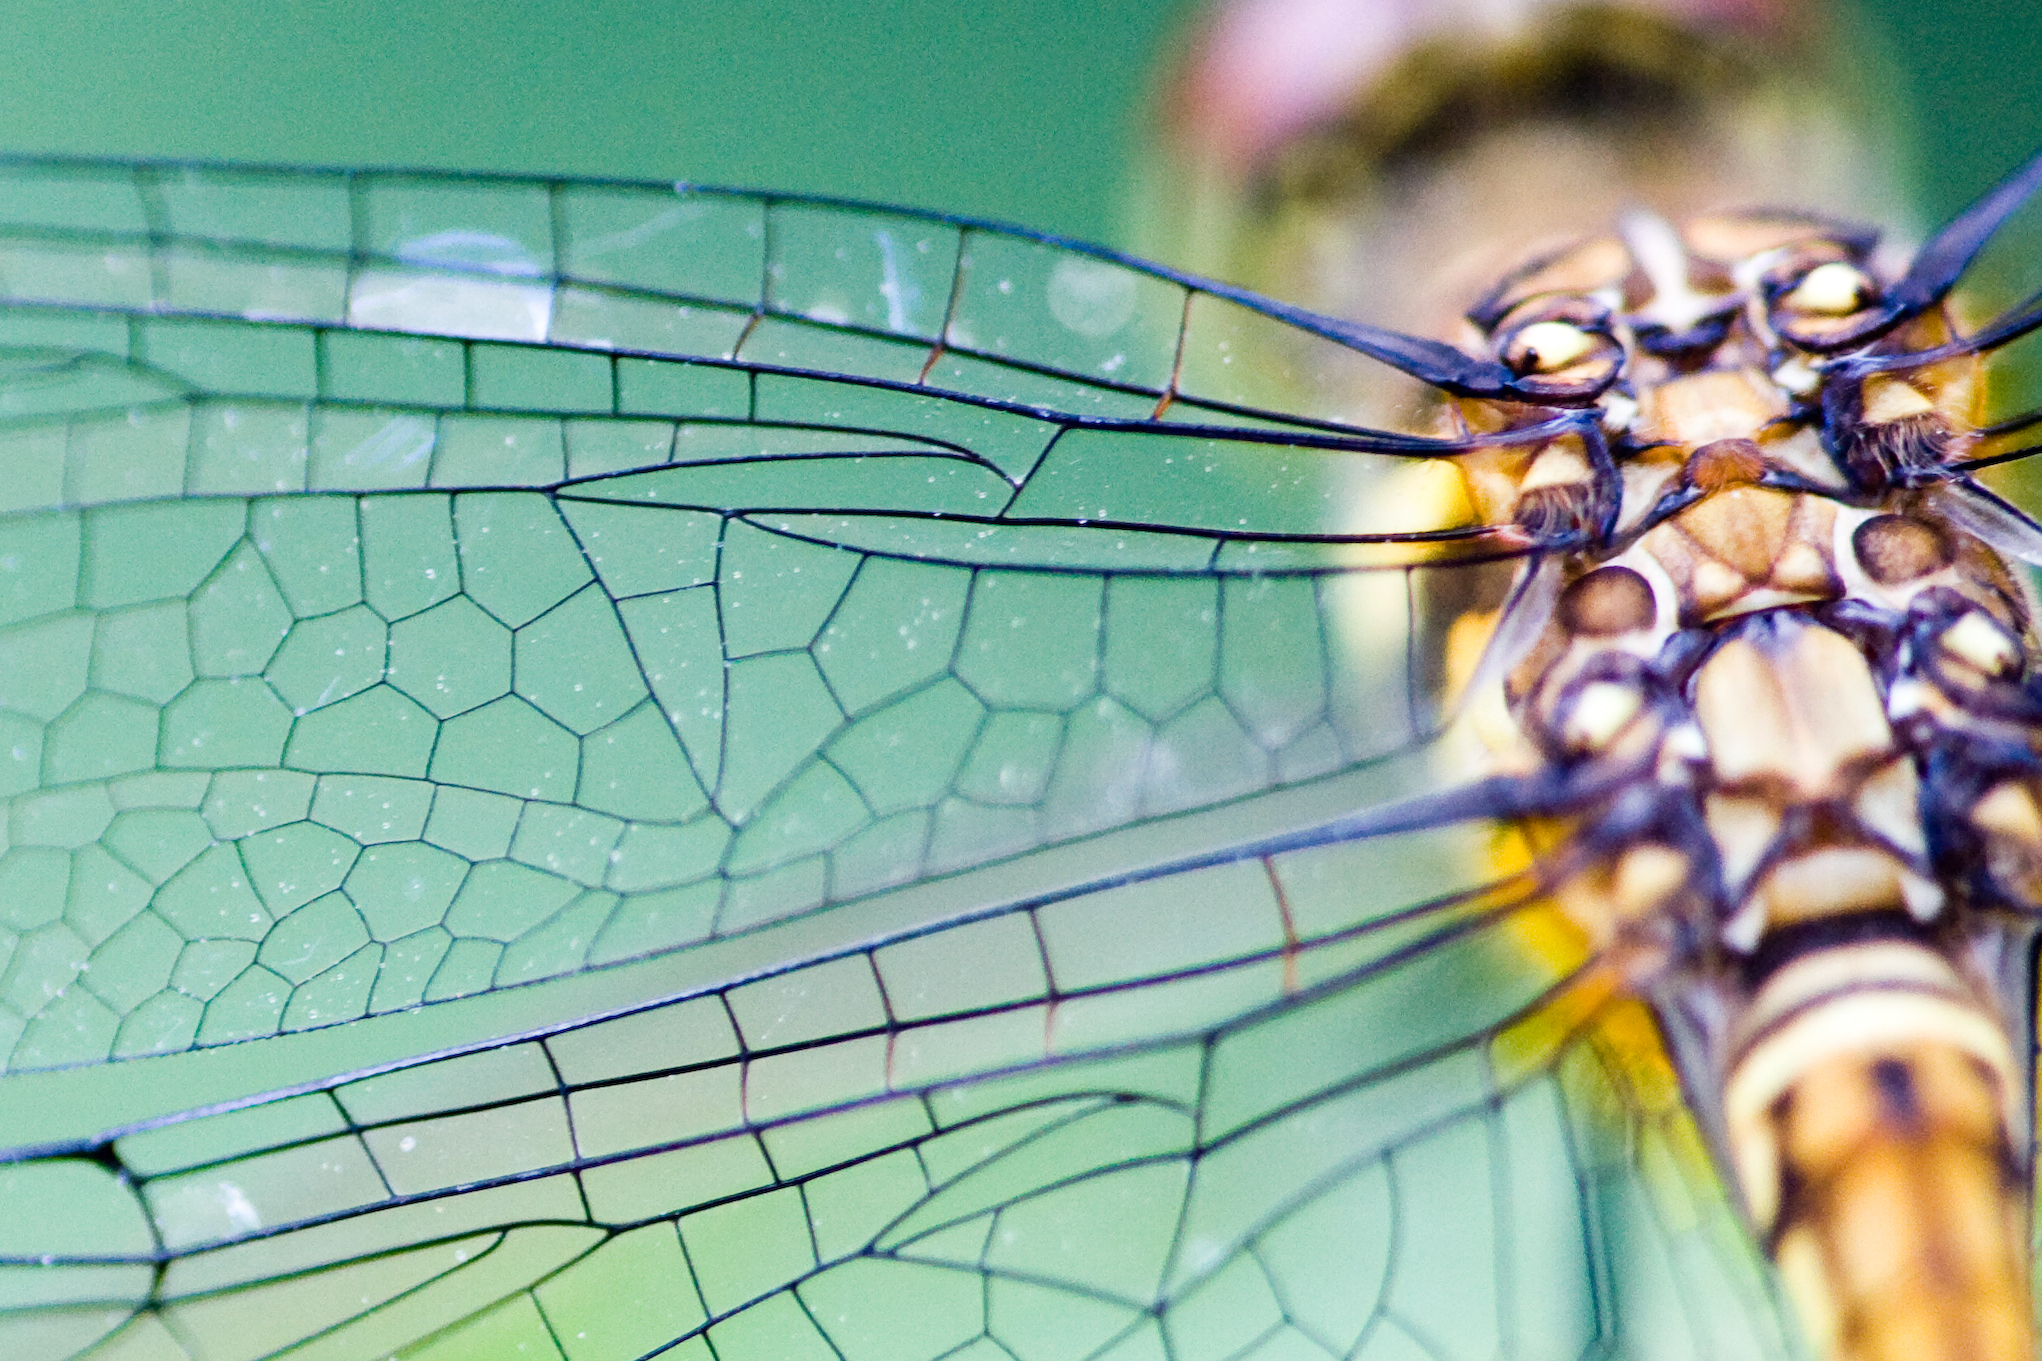
\includegraphics[width=0.7\linewidth]{pics/dragonfly_wing_joi_ito}
	\caption{The wings of a dragonfly. Credit: Joi Ito (CC BY 2.0)}
	\label{fig:dragonflywingjoiito}
\end{figure}



\part{Beyond}

\chapter{A Nontechnical Introduction to NP-Completeness}

\section{The Traveling Salesperson Problem (TSP)}
\section{The Longest Path Problem}
\section{The Rudrata/Hamiltonian Path Problem}
\chapter{Other Data Structures}


\section{Skip Lists}


\chapter{Distributed Hash Tables}



\end{document}